\problemname{Flygildi}

\illustration{0.4}{drone}{Mynd af flygildi eftir \href{https://flic.kr/p/fF81HV}{Richard Unten}}
% \begin{wrapfigure}{r}{0.35\textwidth}
%     \centering
%     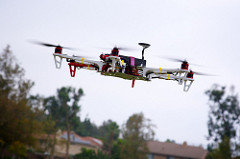
\includegraphics[width=0.32\textwidth]{drone.jpg}
% \end{wrapfigure}

Netverslunin Amazon hefur á síðustu árum verið að þróa nýja leið til að
koma vörum til kaupenda með notkun flygilda\footnote{Flygildi, eða \emph{drone}
á ensku, er lítil sjálfstýrð þyrla.}. Þegar nýja sendingarkerfið er komið í
gang munu viðskiptavinir geta fengið vörurnar sínar afhendar innan örfárra
klukkustunda, í stað þess að bíða í nokkra daga.

Hvert flygildi fær nokkra pakka til að afhenda í einu, og hver pakki hefur
ákveðna staðsetningu sem þarf að afhenda hann á. Svæðið sem flygildin fljúga
yfir er módelað sem tvívítt hnitakerfi, þar sem vöruskemma Amazon er staðsett á
$(0,0)$, og pakka númer $i$ þarf að afhenda á staðsetningunni $(x_i, y_i)$.
Flygildið þarf því að fljúga frá vöruskemmunni yfir á alla afhendingarstaðina í
einhverri röð, og fljúga svo aftur til vöruskemmunnar þegar allir pakkarnir
hafa verið afhentir.

Það er ljóst að röðin sem flygildið heimsækir afhendingarstaðina skiptir miklu
máli, því slæm röð getur þýtt að flygildið fer mun lengri leið til að afhenda
alla pakkana en nauðsynlegt er. Amazon hefur ráðið þig til að leysa þetta
vandamál. Gefinn fjöldi pakka $N$ sem flygildið þarf að afhenda, ásamt
afhendingarstöðunum, hver er stysta leiðin sem flygildið þarf að ferðast frá
því það leggur af stað úr vöruskemmunni, afhendir alla pakkana í einhverri röð,
og þar til það kemur aftur í vöruskemmuna. Gera má ráð fyrir að flygildið geti
flogið beina leið á milli hvaða tveggja punkta sem er án þess að hafa áhyggjur
af árekstrum.

\section*{Inntak}
Fyrsta lína inniheldur heiltöluna $N$ sem táknar fjölda pakka sem þarf að
afhenda. Þar eftir fylgja $N$ línur, ein fyrir hvern pakka. Af þeim mun $i$:ta
línan innihalda tvær heiltölur $-10\,000\leq x_i,y_i \leq 10\,000$, þar sem
$(x_i,y_i)$ táknar staðsetninguna sem þarf að afhenda $i$:ta pakkann á.

\section*{Úttak}
Eina línu með lengdinni á stystu leiðinni sem flygildið þarf að fara. Svarið er
talið rétt ef það er annaðhvort nákvæmlega eða hlutfallslega ekki lengra frá
lengdinni á stystu leiðinni en $10^{-6}$. Þetta þýðir að það skiptir ekki máli
með hversu margra aukastafa nákvæmni svarið er skrifað út, svo lengi sem það er
nógu nákvæmt.

\section*{Útskýring á sýnidæmum}
Í fyrsta sýnidæminu eru bara tveir pakkar. Í þessu tilfelli skiptir ekki máli
hvor pakkinn er afhentur fyrst. Ef flygildið flýgur beinustu leið í hvert
skipti, þá mun lengdin á leiðinni vera $1 + \sqrt{2} + 1 \approx 3.414214$.

\begin{figure}[ht!]
\centering
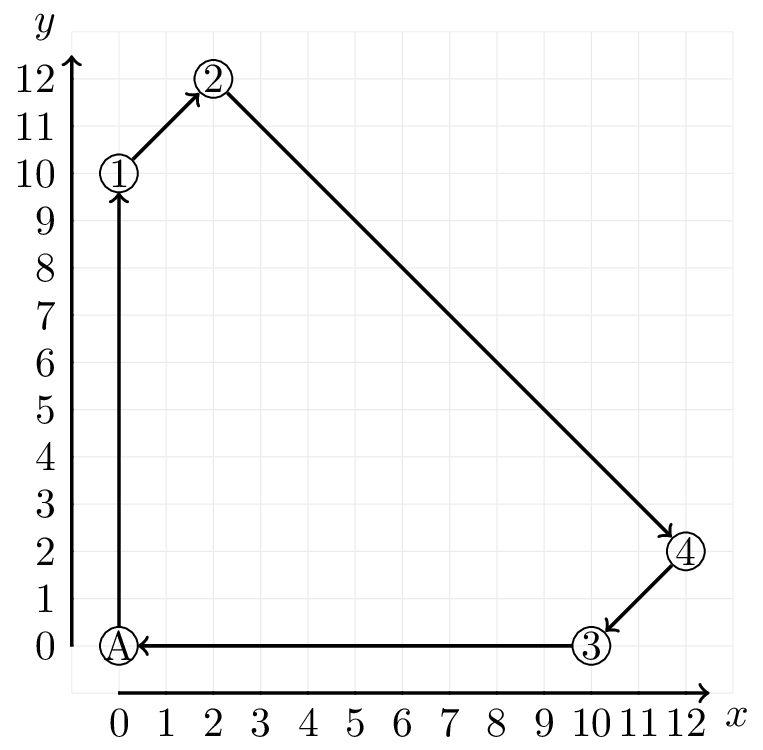
\includegraphics[width=0.4\textwidth]{sample3.png}
\caption{Mynd sem táknar þriðja sýnidæmið.}
\end{figure}

Þriðja sýnidæmið er sýnt í myndinni að ofan. Hér er ljóst að stysta leiðin
afhendir pakkana í röðinni $1$, $2$, $4$, $3$, og gefur það vegalengd sem er
rétt undir $40$.

\section*{Stigagjöf}
Lausnin mun verða prófuð á miserfiðum inntaksgögnum, og er gögnunum skipt í
hópa eins og sýnt er í töflunni að neðan. Lausnin mun svo fá stig eftir því
hvaða hópar eru leystir.

\begin{tabular}{| l | l | l | l |}
\hline
Hópur & Stig & Inntaksstærð & Önnur skilyrði\\ \hline
1 & 10  & $N=1$ & \\ \hline
2 & 10  & $N\leq 3$ & \\ \hline
3 & 20  & $N\leq 1\,000$ & $x_i = 0$ og $y_i \geq 0$ \\ \hline
4 & 20  & $N\leq 1\,000$ & $x_i = 0$ \\ \hline
5 & 40  & $N\leq 8$ & \\ \hline
\end{tabular}
